\documentclass[11pt]{article}
\usepackage{amsmath}
%\usepackage{extsizes}
\usepackage{amsmath,amssymb}
%\usepackage{omegavn,ocmrvn}
%\usepackage[utf8x]{inputenc}
\usepackage[utf8]{vietnam}

\usepackage{framed}
\usepackage[most]{tcolorbox}
\usepackage{xcolor}
\colorlet{shadecolor}{orange!15}


\usepackage{longtable}
\usepackage{answers}
\usepackage{graphicx}
\usepackage{array}
\usepackage{pifont}
\usepackage{picinpar}
\usepackage{enumerate}
\usepackage[top=3.0cm, bottom=3.5cm, left=3.5cm, right=2.5cm] {geometry}
\usepackage{hyperref}


\newtheorem{bt}{Câu}
\newcommand{\RR}{\mathbb R}
\Newassociation{sol}{Solution}{ans}
\newtheorem{ex}{Câu}
\renewcommand{\solutionstyle}[1]{\textbf{ #1}.}


\begin{document}
% \noindent
\begin{tabular*}
{\linewidth}{c>{\centering\hspace{0pt}} p{.7\textwidth}}
Trường ĐHKHTN, ĐHQGHN & {\bf Học Kỳ 1 (2018-2019)}
\tabularnewline
K61 TTƯD & {\bf Kiểm tra cuối kỳ - Đề 2 - Bài mẫu}

\tabularnewline
\rule{1in}{1pt}  \small  & \rule{2in}{1pt} %(Due date:)
\tabularnewline

%  \tabularnewline
%  &(Đề thi có 1 trang)
\end{tabular*}
%
% \Opensolutionfile{ans}[ans1]

\begin{shaded}
Đây chỉ là một mẫu đề thi thầy soạn dựa trên giới hạn của thầy Hiếu, không phải đề thi thật và không có phần nào trùng với đề thi thật.
\end{shaded}

\begin{bt}
	Cho phương trình sau
	%
	\[ 3(2x-1)= \cos(x) \ .\]
	%
	a) Tìm số nghiệm thực và khoảng nghiệm tương ứng của phương trình đó. \\
	b) Hãy viết công thức Newton để giải phương trình trên. Xác định điểm xuất phát $x_0$, 
	hãy tính 3 giá trị đầu tiên $x_i$, $i=1,2,3$. Viết công thức đánh giá sai số hậu nghiệm và áp dụng để 
	đánh giá sai số của $x_3$.
\end{bt}

\begin{bt} Hãy tìm nghiêm của hệ quá xác định $Ax \approx b$ theo nghĩa bình phương tối thiểu bằng một trong hai phương pháp sau với 
%
\[  A = \begin{bmatrix}
1 & 1 \\ 1 & -1 \\ 2 & 1
\end{bmatrix}, \qquad b = \begin{bmatrix}
2 \\ 0 \\ 2
\end{bmatrix}\]
%	
a, Phương pháp lập hệ phương trình chính tắc. \\
b, Phương pháp phân tích QR.
\end{bt}

\begin{bt}
\end{bt}

\begin{center}
	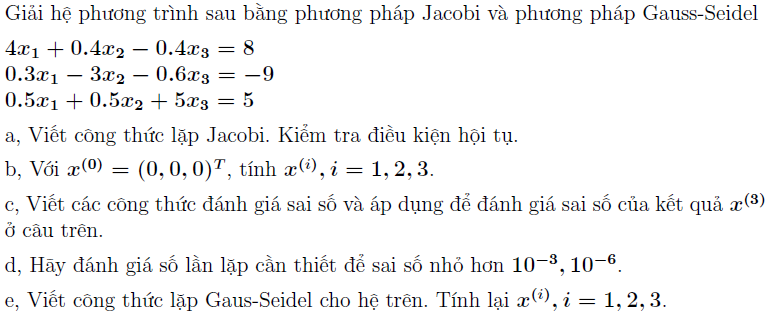
\includegraphics[scale = 0.7]{4}	
\end{center}

\newpage

\begin{bt}
Cho bài toán Cauchy
\end{bt}

\begin{figure}[h!]
	\centering
	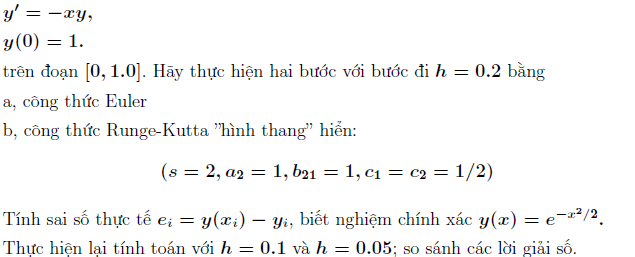
\includegraphics[scale = 0.9]{6}
\end{figure}


\centerline{———————————Hết——————————-}

\end{document}

\vspace{1cm}
\noindent{\bf Chú ý:} {\it Cán bộ coi thi không giải thích gì thêm}\\
\Closesolutionfile{ans}
\newpage
\begin{center}
{\LARGE{\bf ĐÁP ÁN}}
\end{center}

\begin{sol}
	\begin{figure}[h!]
		\centering
		\includegraphics[width=0.8\linewidth]{Solution1/Sol4_1.png}
		%\caption{}
		\label{fig:Sol4}
	\end{figure}
	Exercise 7: Convergence order is 3.	
\end{sol}

   
\end{document}



